\documentclass{article} % For LaTeX2e
\usepackage{nips12submit_e,times}
\usepackage{url,epsfig}
%\documentstyle[nips12submit_09,times,art10]{article} % For LaTeX 2.09


\title{Image Classification with MLP and CNN}


\author{
Bo Tian \\
No. 2012011346,
Tsinghua University \\
\texttt{dxmtb@163.com} 
}

\nipsfinalcopy % Uncomment for camera-ready version

\begin{document}

\renewcommand{\arraystretch}{1.3}

\maketitle

\section{Introduction}

Recently machine learning methods involving neural networks are very popular and mostly achieve states of the art performances. In this report I will present my experiments on Multilayer Perceptron and Convolution Neural Network. I tried to use both of them to classify images on CIFAR-10 dataset, and compared different hyper-parameters. And I will introduce how to implement an efficient convolution neural network.

Finally, I got 70.52\% classification accuracy with codes written in Python and C++ on CIFAR-10 dataset. About 150 images can be processed with a CPU and about 400 images with a GPU. Because I implemented all funtionality myself, the results are comparable to the results provided by MATLAB codes (about 75\%).

In section~\ref{sec:Models}, I will briefly introduce the models I used. Section~\ref{sec:Experiments} introduces the experiment setup and the results I got, and some analysis will be given. Finally, I will introduce some tricks to implement a fast convolution neural network in section~\ref{sec:Implementation}.

\section{Models}

\label{sec:Models}

\subsection{MLP}

Multilayer Perceptron (MLP), which consists one input layer, one hidden layer and one output layer, is one of the simplest neural network. The output of a fully connected layer is given by

$$y=f(Wx+b)$$

where $x$ is the input, $W$ and $b$ are parameters for current layer, and $f$ is the activation function, which may be tanh, sigmoid or ReLU. MLP is the stack of two fully-connected layer.

Feeding images to a MLP, it is supposed to output the classes of the images. Assuming that we have $K$ classes, the expected output vector $y$ should have $y_i=1$, where $i$ is the index of the correct class, and $y_j=0$ where $j\neq i$. 

There are two kinds of training objectives. Let $t_i$ be the standard output of the $i^{\mbox{th}}$ input, $N$ be the number of training samples. Least square error objective is to minimize

\begin{equation}
J(\theta)=\frac{1}{2}\sum_{i=1}^N (t_i-y_i)^2
\end{equation}

and cross-entropy error objective is to minimize

\begin{equation}
J(\theta)=-\sum_{i=1}^N t_i \ln{y_i}
\end{equation}

where $\theta$ is the parameter of the model.

Usually a softmax layer is concatenated when cross-entropy error is used. Softmax layer produces the output

\begin{equation}
y_i=\frac{e^{z_i}}{\sum_{j=1}^K e^{z_j}}
\end{equation}

where $z=Wx+b$ and $x$ is the input from former layer.

We call $J(\theta)$ error function. Taking the gradients of error function, we can use stochastic gradient descent (SGD) to train a network.

\subsection{CNN}

Another more complicated model is Convolution Neural Network (CNN). The input to a convolution layer is a set of 2D matrixes called feature map. By convolving feature maps with several shared filters, a output consisting another set of 2D matrixes is produced. Formally, the output of a convolution layer is

\begin{equation}
	y_q = f(\sum_{p \in {M_q}} x_p * \mbox{rot180}(w_{qp}))
\end{equation}

where $y_q$ is the output of current layer, $x_p$ is the input from former layer, $f$ is the activation function, $M_q$ denotes a selection of input maps in former layer. $*$ here is valid convolution.

Usually a max pooling layer is followed right after a convolution layer. A maximum pooling layer outputs only the maximum values in 2D windows. The width or height of a pooling window is usually 2 or 3. It intends to reduce the size of feature maps.

\subsection{Dropout} % (fold)
\label{sub:dropout}

Dropout~\cite{Bell} is a regularization technique. In the training process, the output of each neuron is set to zero with probability 0.5 (not including output layer). These neurons set to zero won't contribute to both forward and backward pass. It is easy to implement and can avoid over-fitting. When testing, we will multiply all the outputs of neurons by 0.5 to reduce the effect of dropout.

It usually shows better performance as the network is like a combination of many networks randomly selected from 50\% of the network, which have the full capability to do the classification.

% subsection dropout (end)

\section{Experiments}

\label{sec:Experiments}

\subsection{The Dataset}

I use the CIFAR-10 dataset~\cite{Krizhevsky} in all our experiments. The CIFAR-10 dataset consists of 60000 32x32 color images in 10 classes, with 6000 images per class. There are 50000 training images and 10000 test images. 

The dataset is divided into five training batches and one test batch, each with 10000 images. The test batch contains exactly 1000 randomly selected images from each class. The training batches contain the remaining images in random order, but some training batches may contain more images from one class than another. Between them, the training batches contain exactly 5000 images from each class.

I will use the fifth training batch as validation batch for tuning hyper-parameters.

\subsection{Results and Analysis}


\subsubsection{MLP}

Our results of MLP are summarized in Table~\ref{MLP}.

\begin{table} [h]
\caption{ {\it Comparison of results with different objectives and activation functions}}
\vspace{2mm}
\centerline{
\begin{tabular}{|c|c|c|c|}
\hline
Objectives and activation & tanh & sigmoid & ReLU\\
\hline
Least Square Error & \textbf{52.95}\% & 35.78\% & 52.79\%\\
\hline
Cross-Entroy Error & 50.11\% & 41.87\% & 50.77\%\\
\hline
\end{tabular}
}
\label{MLP}
\end{table}

For each combination of objective and activation function, a few hyper-parameters including different sizes of layers and learning rates were tried, and then the models were train with training batches exclude validation batch for 20 epochs. Then I chose the hyper-parameters with the best performance on validation batch and trained the model with all five training batches for 100 epochs. Finally, I did testing on test batch.

Most of the models achieved best performance with 1600-dimension hidden layer, and learning rate 0.00001, momentum rate 0.9, and weight decay rate 0.003.

The following graph shows testing accuracy during training.

\begin{figure}[h]
	\centering
		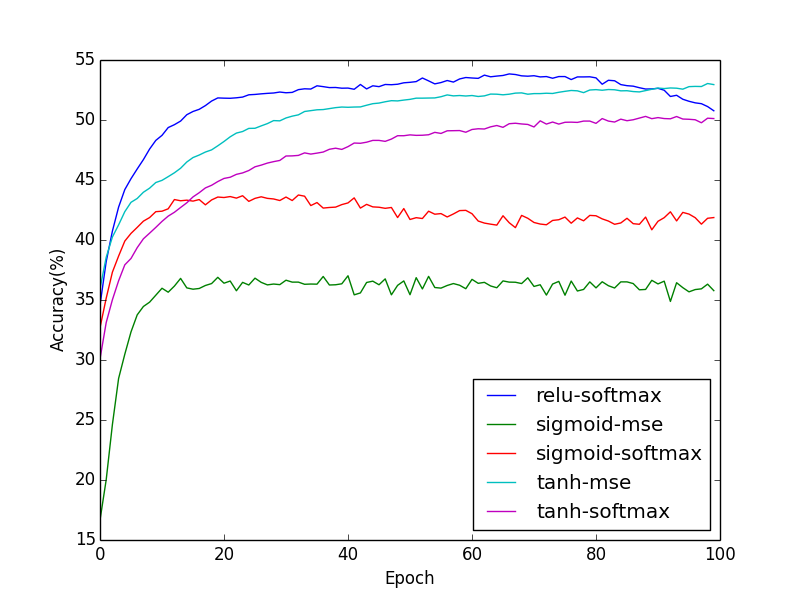
\includegraphics[width=.9\textwidth]{mlp.png}
	\caption{Testing Accuracy during Training}
	\label{fig:mlp}
\end{figure}

We can see for sigmoid activation, the testing accuracy achieve best at about epoch 15, and after that it almost remains unchanged. In the beginning, the ReLU with softmax model always performs better. After epoch 80, it is over-fitting and the testing accuracy drops. The performance of tanh with minimum square error objective model can be better if we train another a few epochs. Roughly, ReLU is very suitable for problems like image classification. 


\subsubsection{CNN}

Our results of CNN are summarized in Table~\ref{CNN}.

\begin{table} [h]
\caption{ {\it Comparison of results with different objectives and activation functions}}
\vspace{2mm}
\centerline{
\begin{tabular}{|c|c|c|c|}
\hline
Objectives and activation & tanh & sigmoid & ReLU\\
\hline
Least Square Error & 36.38\% & 61.74\% & \textbf{70.52}\%\\
\hline
Cross-Entroy Error & 62.61\% & - & 69.65\%\\
\hline
\end{tabular}
}
\label{CNN}
\end{table}

There are two convolution layers with two max-pooling layers followed by a fully connected layer and 32 feature maps in each convolution layer. The size of filters is 5x5 and pooling size is 2. 

I used the method described in last section to choose hyper-parameters. Then, the training methodology is similar to that described in~\cite{cuda-convnet}. To achieve the best results, I trained on training batches not including validation batch until validation error stops improving. After that I trained with validation batch until training error reaches almost the same value. Finally, I reduced learning rates by 10 times and trained for another 10 epochs for a second time.

For the limitation of time I didn't manage to tune hyper-parameters for every model but only ReLU-Softmax model. All the other models used hyper-parameters from ReLU-Softmax model and achieved acceptable performance. For the combination of sigmoid activation function and cross-entropy error, I didn't find feasible hyper-parameters.

The following graph shows negative testing log likelihood during training.

\begin{figure}[h]
	\centering
		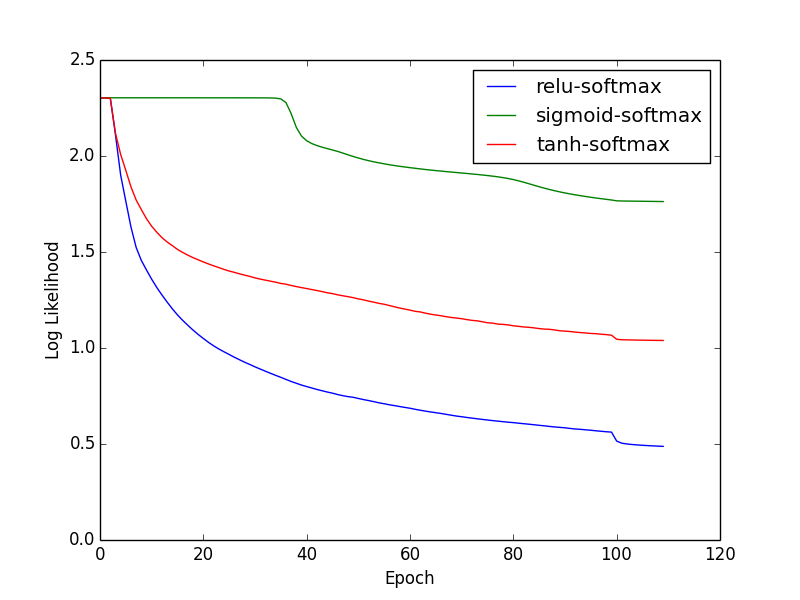
\includegraphics[width=.9\textwidth]{cnn.png}
	\caption{Negative Log Likelihood during Training}
	\label{fig:cnn}
\end{figure}

The speed of the decreasing of negative log likelihood slowed down when epoch number increased. After epoch 100, I reduced the learning rate, so that it decreased faster. What is interesting is that the model sigmoid-softmax keeps unchanged at the first 40 epochs, and started decreasing as normal after that. I guess it is because the initial value wasn't very good and after a series of descent it jumped out of the bad value. It also shows that it is not always bad when you don't see any improvements at the beginning epochs.

In order to improve performance, we need more layers and a better gradient descent algorithm, such as AdaGrad. We can use different strides in convolution and pooling. If we don't use overlapped pooling window, we can stack at most two conv-pooling layers. But too many layers will make the computation expensive.

\section{Details of Implementation}

\label{sec:Implementation}

The main framework of my code is on Python. The biggest difficulty is how to implement an efficient CNN with Python not so efficient. In the following sections I will describe a few challenges and address the solutions.

\subsection{Fast Convolution}

In the earlier version of codes, the convolution is implemented with scipy.signal.convolve2d, but it is extremely slow. I also tried FFT that guarantee better time complexity but actually it is slow because filters are very small. At last, I found conv2d in theano is very efficient, and can be accelerated with a GPU with CUDA.

The table~\ref{conv} shows running time of 2D convolutions between batches of several feature maps and several filters, which intend to simulate a forward process. With scipy, we can only convolve two 2D matrixes at one time, and iterations are needed to get the final output. The function provided by theano can do 2D convolution between two 4D matrixes directly, which can be much faster.

\begin{table} [h]
\caption{ {\it Comparison of running time (seconds) with different tools and tasks}}
\vspace{2mm}
\centerline{
\begin{tabular}{|c|c|c|}
	\hline
	Tools and Tasks     & single & conv 2d \\
	\hline
  GPU (theano) & 0.3485 & \textbf{0.0135} \\
	\hline
	CPU (python) & 0.2754 & 2.4587 \\
	\hline
  CPU (theano) & \textbf{0.0665} & 0.1503 \\
\hline
\end{tabular}
}
\label{conv}
\end{table}

The batch size I used is 100, and each input contains 3 feature maps with size 32x32. There will be 32 output feature maps so there are 32x3 filters with size 5x5.

The column single means the time running one single 2D convolution. The column conv 2d means the time running 2D convolution between two 4D matrixes. It shows when doing single 2D convolution, theano on CPU is fastest. And when doing conv 2D, theano on GPU is 245x faster than scipy version and 15x faster than theano on CPU version. So I choose to use theano for doing convolution.

In more detail, a fast convolution function for CNN will first rearrange all blocks of input feature maps into columns (i.e. im2col), and respectively construct filter matrixes with filter on each column. Although the construction maybe slow, but the convolution done by General Matrix-Multiply (GEMM) is very efficient finally.

\subsection{Fast Pooling}

Pooling is implemented with C++ code to get efficient indexing. Python can use ctypes to call C library. The gradient of pooling can be implemented in a similar way. There is no trick but using pointers carefully.

\subsection{Fast Rotation}

In several cases, we need to do rot180 for last two dimensions of a 4D matrix. The intuition is to do rot90 twice for each 2D matrix and construct a 4D matrix, but this is slow. The fancy indexing of numpy can help with this, we can simply write ``tensor[:,:,::-1,::-1]''. Because numpy doesn't move memory when doing indexing, so it almost cost nothing.

\subsection{Fast Gradient Computation}

Because I didn't use gradient computation of theano, I have to compute gradient by my codes. The gradient of $W$ is

\begin{equation}
	\frac{\partial J}{\partial W_{q,p}} = \sum_{i=1}^N y_{i, p} * R(\delta_{i, q})
\end{equation}

where $W$ is parameter for current layer, N is the batch size, $y_{i,p}$ is the $p^{\mbox{th}}$ feature map of the $i^{\mbox{th}}$ input, R stands for rotation for 180 degrees, and $\delta_q$ is the local sensitivity from the $q^{\mbox{th}}$ feature map of the $i^{\mbox{th}}$ output. 

Using the formula above, it needs 3 loops, which can cost a lot of time. We hope to make use of theano conv2d.

After inspecting into the formula, we can find that $i$ can be regarded as the index of input feature maps, let $y'_{i,j}=y_{j,i}$, $R(\delta'_{i, j})=R(\delta_{j, i})$, then

\begin{equation}
	\frac{\partial J}{\partial W_{q,p}} = \sum_{i=1}^N y'_{p, i} * R(\delta'_{q, i})
\end{equation}

which is exactly what theano conv2d wants to do as following

\begin{equation}
	\frac{\partial J}{\partial W} = \mbox{conv2d}(y', R(\delta'))
\end{equation}

A similar optimization can be applied when computing local sensitivity.

\section{Conclusion} % (fold)
\label{sec:conclusion}

I implemented both MLP and CNN with Python and C++ and the models achieved acceptable performance. How to select hyper-parameters, how they affect performance and how to implement a fast neural network is also discussed in this report.

% section conclusion (end)

\bibliography{strings,refs}

\begin{thebibliography}{10}

\bibitem{Krizhevsky} Krizhevsky, Alex, and Geoffrey Hinton. Learning multiple layers of features from tiny images. Computer Science Department, University of Toronto, Tech. Rep (2009).
\bibitem{Bell} R.M.Bell and Y.Koren.Lessons from the netflix prize challenge. ACM SIGKDD Explorations Newsletter, 9(2):75–79, 2007.
\bibitem{cuda-convnet} Krizhevsky. cuda-convnet Methodology. URL \\
  https://code.google.com/p/cuda-convnet/wiki/Methodology.


\end{thebibliography}

\end{document}


